
\documentclass{article}
\usepackage[utf8]{inputenc}

\title{Bayesian Optimization}
\author{Simone Tibaldi}
\date{March 2021}

\usepackage{natbib}
\usepackage{amsmath}
\usepackage{parskip}
\usepackage{amsfonts}
\usepackage{graphicx}
\usepackage{subcaption}
\graphicspath{ {./images/} }

\begin{document}

\maketitle

\section{Introduction}
All the materials and consideration over Bayesian Otpimization tasks

\section{Gaussian Procesesses and Bayesian Optimization}

\subsection{MultiVariate Normal (MVN) Distributions}
A variable that follows a normal distribution has a probability density function (PDF) given by the Gaussian distribution with mean $\mu$ and variance $\sigma$.
\begin{equation}
    \mathcal{N}(x | \mu, \sigma) = C \text{e}^{-\frac{1}{2} \frac{(x-\mu)^2}{\sigma^2}}
\end{equation}
A bi-dimensional normal distribution on two variables $x_1, x_2$ needs a 2D mean vector $\mathbf{\mu}$ and a covariance matrix $\Sigma$ as variance. Each entry of the matrix $\Sigma_{ij}$ is the covariance of variable $i$ with variable $j$ and the diagonal elements, \textit{i.e.} $K_{ii}$, are just the variances of the single variables. So in general: 
\begin{align*}
    \Sigma_{ij} = \frac{\sigma(x_i, x_j)}{\sigma(x_i)\sigma(x_j)} 
\end{align*}
with $\sigma(x_i) = \sqrt{\mathbb{E}(x_i - \mu)^2}$ being the expectation of variable $x_i$ and $\sigma(x_i, x_j) =  \mathbb{E}(x_i - \mu_i)(x_j - \mu_j)$, which means that all entries are in the range [0 1] where 1 means that they are fully correlated, \textit{i.e.} $x_1$ is equal to $x_2$, and 0 means totally uncorrelated, \textit{i.e.} sparse w.r.t. each other. The variance matrix $\Sigma$ is always symmetric and semi-definite positive.

\begin{figure}
    \centering
    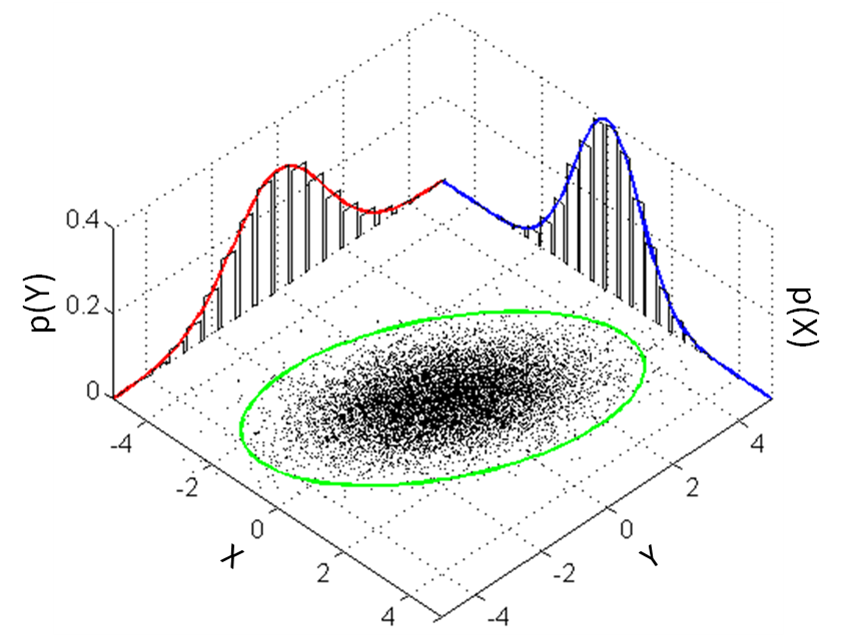
\includegraphics[width = .7\linewidth]{mvn2d.png}
    \caption{3D representation of a two dimensional Gaussian distribution. The scattered points follow the normal distribution $P(x)$ along the $x$ and $P(y)$ along $y$, both obtained by summing over the other variable.}
    \label{mvn2d}
\end{figure}

For example in Figure \ref{mvn2d} the correlation matrix is
\begin{align*}
    \Sigma = 
    \begin{bmatrix}
    1, & .5 \\
    .5 & 1
    \end{bmatrix}
\end{align*}
meaning that the two variables are correlated to each other. If the off-diagonal elements are zeros every variable is independent from the others and the 2D Gaussian has a circular shape at the base and is the same when looked from every direction. 

\paragraph{Multi Variate Normal Distributions Theorem}
The \textit{joint distribution} of the two variables is given by:
\begin{equation}
    p(x_1, x_2) \propto e^{-\frac{1}{2}(\mathbf{x}^T \Sigma \mathbf{x})}
\end{equation}
where $\mathbf{x} = (x_1, x_2)$. In addition to that we have the:
\begin{itemize}
    \item \textit{Conditionals} (or posterior conditionals) $p(x_1) = p(x_1 | x_2 = x_2^*)$ and $p(x_2) = p(x_2 | x_1 = x_1^*)$ which are obtained by fixing one of the two variables (in the starred points) and see how the other is distributed. The conditionals in 2D normal distributions can be visualized as cutting a slice of the Normal distribution and watching only one side. 
    \item \textit{Marginals} $p(x_1), p(x_2)$ are obtained by tracing out (summing over) the other variable. That is also shown in the Figure \ref{mvn2d}.
\end{itemize} 
In general, if there is no correlation $\Sigma_{12} = \Sigma_{21} = 0$ then there is no way to obtain any information on $x_1$ by picking a value of $x_2$ and viceversa. 

The Marginals and Conditionals are obtained through the Theorem for MVN's. For a BiVariate  normal distribution with mean and covariance:
\begin{equation}
    \mu =
    \begin{bmatrix}
    \mu_1 \\
    \mu_2
    \end{bmatrix},
    \quad
    \Sigma = 
    \begin{bmatrix}
    \Sigma_{11} & \Sigma_{12} \\
    \Sigma_{21} & \Sigma_{22} 
    \end{bmatrix},
    \quad
    \Lambda = \Sigma^{-1}
\end{equation}
we can calculate:
\begin{enumerate}
    \item Marginals:
    \begin{align}
        p(x_1) = \mathcal{N}(x_1 | \mu_1, \Sigma_{11}) \\
        p(x_2) = \mathcal{N}(x_2 | \mu_2, \Sigma_{22}) 
    \end{align}
    \item Conditionals:
    \begin{align}
        p(x_1 | x_2) &= \mathcal{N}(x_1 | \mu_{1|2}, \Sigma_{1|2}) \\
        \mu_{1|2} &= \mu_1 + \Sigma_{12} \Sigma_{22}^{-1}(x_2 - \mu_2) \\
        \Sigma_{1|2} &= \Sigma_{11} - \Sigma_{12}\Sigma_{22}^{-1}\Sigma_{21} = \Lambda^{-1}_{11}
    \end{align}
\end{enumerate}

\paragraph{Generalization to $N$ Dimensions}
For $N$ variables normally distributed we can create a joint Multi Variate Normal distribution $f(x_1, \dots, x_N)$ that we write as:
\begin{equation}
    \begin{bmatrix}
    f(x_1) \\
    f(x_2) \\
    \vdots \\
    f(x_N)
    \end{bmatrix}
    \sim
    \mathcal{N}
    \begin{pmatrix}
    \begin{bmatrix}
    \mu_1 \\
    \mu_2 \\
    \vdots \\
    \mu_N
    \end{bmatrix}
    ,
    \begin{bmatrix}
    \Sigma_{11} & \Sigma_{12} & \dots & \Sigma_{1N} \\
    \Sigma_{21} & \Sigma_{22} & \dots  \\
    \vdots & \vdots{} & \ddots \\
    \Sigma_{N1} & \dots & \dots & \Sigma_{NN}
    \end{bmatrix}
    \end{pmatrix}
\end{equation}
To calculate marginals and conditionals the generalization from the 2D case is pretty straightforward, considering a set of normally distributed variables $X = {x_1, \dots x_N}$ with means $\mu_1, \dots, \mu_N$ and covariance matrix $\Sigma$:
\begin{itemize}
    \item Marginals: the marginal of any subset $S$ of $X$, $S \subset X$ is obtained by the Multivariate Normal distribution of the variables in $X - S$
    \item Conditionals: By recasting $X$ as a 2D vector $X = [\boldsymbol{x}_1, \boldsymbol{x}_2]$ where $\boldsymbol{x}_1$ has $q$ elements and $\boldsymbol{x}_2$ has $N-q$ elements (same reasoning goes for $\mu$ and $\Sigma$) we have the same equations
    \begin{align}
        p(\boldsymbol{x}_1 | \boldsymbol{x}_2) &= \mathcal{N}(\boldsymbol{x}_1 | \boldsymbol{\mu}_{1|2}, \boldsymbol{\Sigma}_{1|2}) \\
        \boldsymbol{\mu}_{1|2} &= \boldsymbol{\mu}_1 + \boldsymbol{\Sigma}_{12} \boldsymbol{\Sigma}_{22}^{-1}(\boldsymbol{x}_2 - \boldsymbol{\mu}_2) \\
        \boldsymbol{\Sigma}_{1|2} &= \boldsymbol{\Sigma}_{11} - \boldsymbol{\Sigma}_{12}\boldsymbol{\Sigma}_{22}^{-1}\boldsymbol{\Sigma}_{21} = \boldsymbol{\Lambda}^{-1}_{11}
    \end{align}
    where $\boldsymbol{\Sigma}_{11}$ is created only with the variables of the subset $\boldsymbol{x}_1$, so it has dimensions $q \times q$, same for the other terms. 
\end{itemize}
In particular the calculation of the variance and mean for the conditionals requires the computation of the inverse of $\Sigma$. This is typically done with the Cholensky Decomposition. 

On a final note, to visualize in 2 Dimensions we can project the points of the 2D Gaussian into a plane where the $x$-axis has the two variables as two separated discrete values and in the $y$-axis the values that the two variables have at a specific point, Figure \ref{visual}. 
\begin{figure}
    \centering
    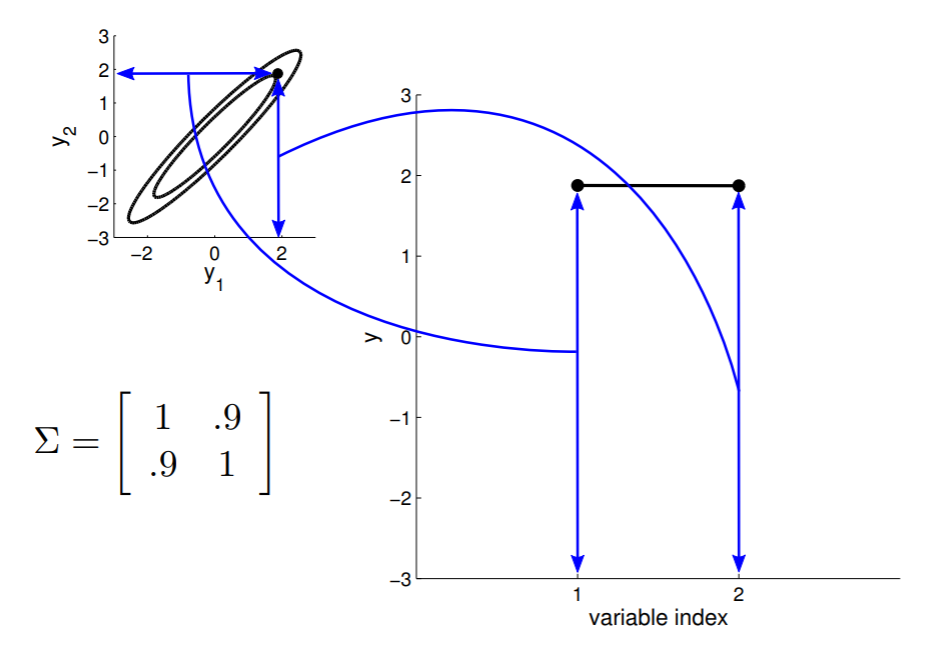
\includegraphics[width = .8\linewidth]{visualize1.png}
    \caption{Visualizing a 2D Gaussian on a plane. Every point in the upper left panel is drawn from a 2D normal distribution with the covariance matrix in the bottom left corner. The selected point has coordinates $(2,2)$ and so both dimensions on the $x_1, x_2$ (represented on the horizontal axis) have corresponding value 2.}
    \label{visual}
\end{figure}

This helps us generalize to $N$ dimensions \footnote{Very helpful checking out this page: https://thegradient.pub/gaussian-process-not-quite-for-dummies/} where we can set the variables $x_1, x_2, \dots x_N$ on the $x$-axis and the values of a single $N$-dimensional point on the $y$-axis, each of its coordinates is the ordinate of the corresponding variable. Connecting the values forms a shape that can be interpreted as a function of the discrete variables $x_1, x_2, \dots x_N$. An example for the case of a 5D Normal distribution is shown in Figure \ref{example}. The shape of the covariance matrix $\Sigma$ from which we draw the points is crucial in deciding the shape of this "function" that connects the variables. In fact variables that are highly correlated (close to 1) tend to have very similar values, viceversa for variables with low covariance. This implies that if we create a covariance matrix with values close to 1 for variables that we consider close in the $x$-axis and values close to 0 for variables that are far away we are asking the shape of our "function" to be as smooth as possible, or continuous in some sense. This is exactly the starting idea, or prior, of the Gaussian Process. For example consider Figure \ref{example} where $\Sigma$ has decreasing variances for distant points. This allows the "function" of every sampled point to be "smooth" (as smooth as a discrete function can be).

\begin{figure}
    \begin{subfigure}{.5\textwidth}
      \centering
      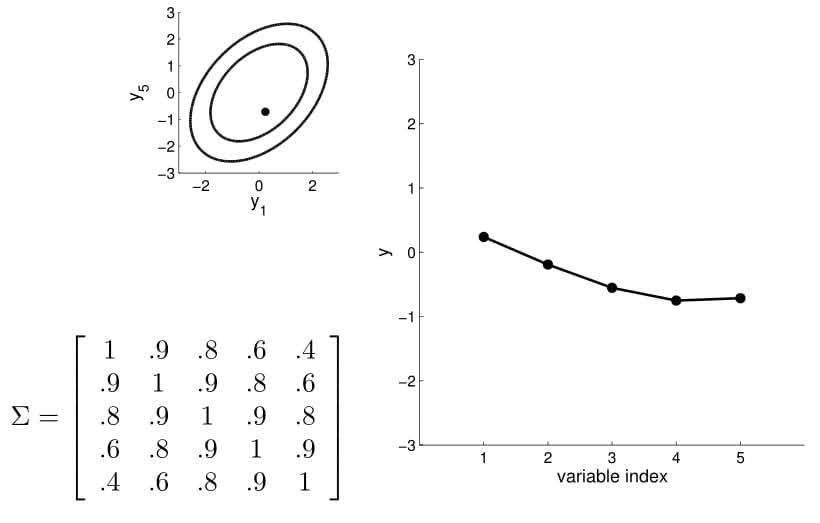
\includegraphics[width=\linewidth]{gauss5d1.jpg}
      \caption{1a}
      \label{fig:sfig1}
    \end{subfigure}%
    \begin{subfigure}{.5\textwidth}
      \centering
      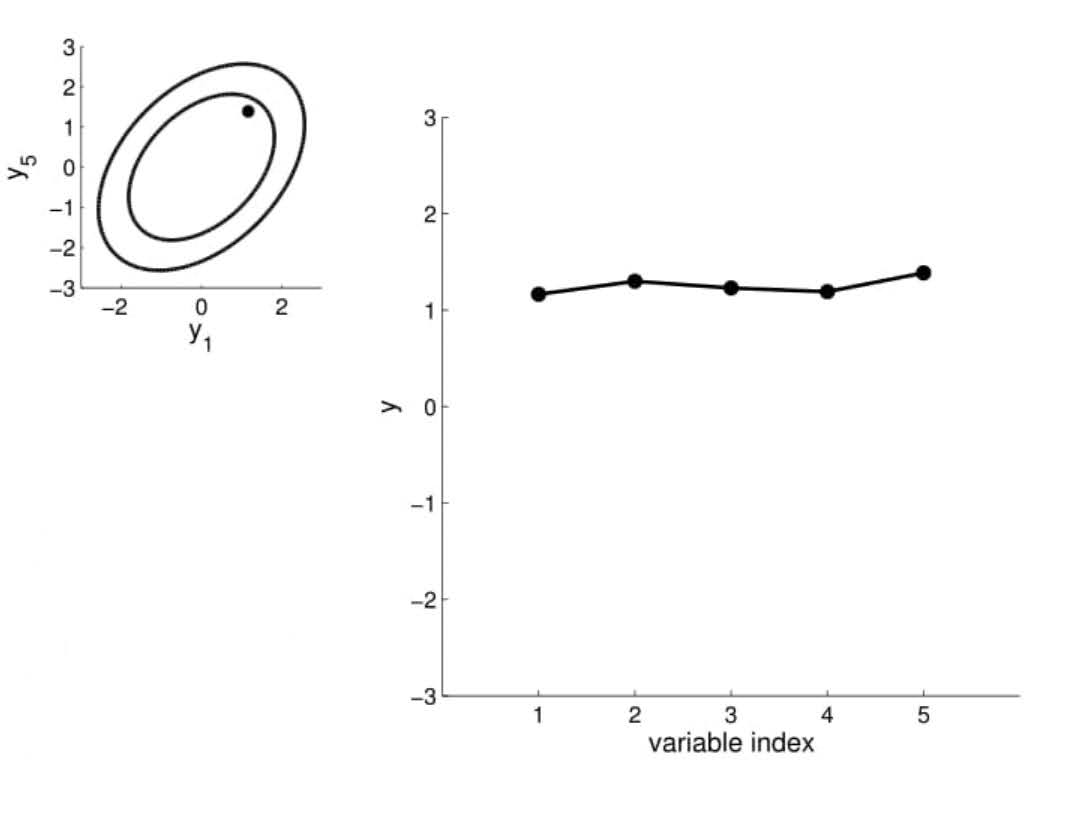
\includegraphics[width=\linewidth]{gauss5d2.jpg}
      \caption{1b}
      \label{fig:sfig2}
    \end{subfigure}
    \caption{Two dimensional representation of two points extracted from a 5 dimensional normal distribution. The first two dimensions of the extracted points are shown in the top left corner, the dots correspond to the sampled points. By picking the 5 values of each variable and plotting them on the right we obtain a function over the 5 discrete variables.}
    \label{example}
\end{figure}

\subsection{Gaussian Processes}
A GP is a regression model used to estimate a (usually unknwown and complicated) function or to calculate its minima/maxima. The initial assumption is that we have a set of datapoints $\mathcal{D} = \{(x_{TR}, f(x_{TR}))\}$ where $x_{TR}$ can be called Training points where we sample the function (which might be expensive to evaluate) and $f(x_{TR})$ is the corresponding value of the function. The objective of the procedure is to reconstruct the function. In particular we want a process that, given the dataset $\mathcal{D}$ and a new set of test points $x_{TE}$, can estimate the most probable values $f(x_{TE})$ and most importantly tells us how confident we are about those values (this is intuitively shown in Figure \ref{gp} where the shaded areas mean low confidence on the values of the function).

The GP relies on one main assumption: every training point at which we sample the function and every points at which we test the function (to know its probable value and our uncertainty about it) is considered as a random variable with its own normal distribution. This means that the training and test variables altogether form a multivariate normal distribution. This allows us to sample points from this distribution that, with help from the visualization scheme of the previous section, can be considered as functions over the train and test variables. The Gaussian Process is created in a way that makes the sampled functions pass exactly at each point of the training set, meaning that for each of the $x_{TR}$ it will have value \textit{i.e.} $f(x_{TR})$, while for the test variables it can only produce a mean value and variance each that we use as most likely value and uncertainty about such value. 

So in practice, we exploit a bayesian procedure that starts with a gaussian prior. The prior is a family of functions sampled from a multivariate normal distribution with, usually, mean 0. So every function we sample from the starting prior has mean 0 and is randomly distributed around this value, meaning they are completely random functions. Then we use our training set $\mathcal{D}$ to update our belief on the function $f$ given our data, \textit{i.e.} p(f, $\mathcal{D})$, by Bayes rule as usual
\begin{equation}
    p(f | \mathcal{D}) \propto p(\mathcal{D} | f) p(f)
\end{equation}
This is the point where we enforce our normally distributed functions to pass from the points $f(x_{TR})$.

\paragraph{Gaussian Prior}
The prior of a Gaussian Process assumes that the variables from which we sample the unknown function is a set of variables that are normally distributed and thus form a Multi Variate Normal (MVN) distribution. This is done for two reasons:
\begin{itemize}
    \item Every value of $x$ has an associated mean $\mu(x)$ and variance $\sigma(x)$. This is exactly what we want because it allows us to tell what is our current belief on the value of $f(x)$, given by $\mu(x)$, and how confident we are about it, given by the variance $\sigma(x)$. The starting value for the mean is 0 for every variable. 
    \item We can create an ad hoc correlation matrix $\Sigma$ that gives a preferred shape to the prior
\end{itemize}
This means that at every iteration of the GP our current belief on what $f$ looks like can be obtain by sampling the MultiVariate Normal distribution at $N$ values of $x$. Since each variable have their own mean and variance we can connect the sampled values to form a random function. Repeating the sample we create a family of random functions and the mean and variance of this family of functions tells us how much we know about $f$. This becomes more intuitive with the help of the visualization procedure of Figure \ref{visual2}, where we have a 20 MVN and we sample the values of the first two variables. Since these values are now clamped they cannot change , they are fixed by the sampling and the Bayesian step
. Instead, the following values of the remaining 18 variables are distributed according to (for each one) their own mean $\mu_i$ and variance $\Sigma_{ii}$. The more we move away from the clamped values the harder it gets to predict the value of the variable if we sample from its distribution (because covariance gets smaller between distant variables). So if now we sample from this 20 normally distributed variables we get a set of functions that always passes from the first two points and then randomly oscillates around the mean $\mu_\star$ with variance $\Sigma_\star$. This is the shape of our prior. 

\begin{figure}
    \centering
    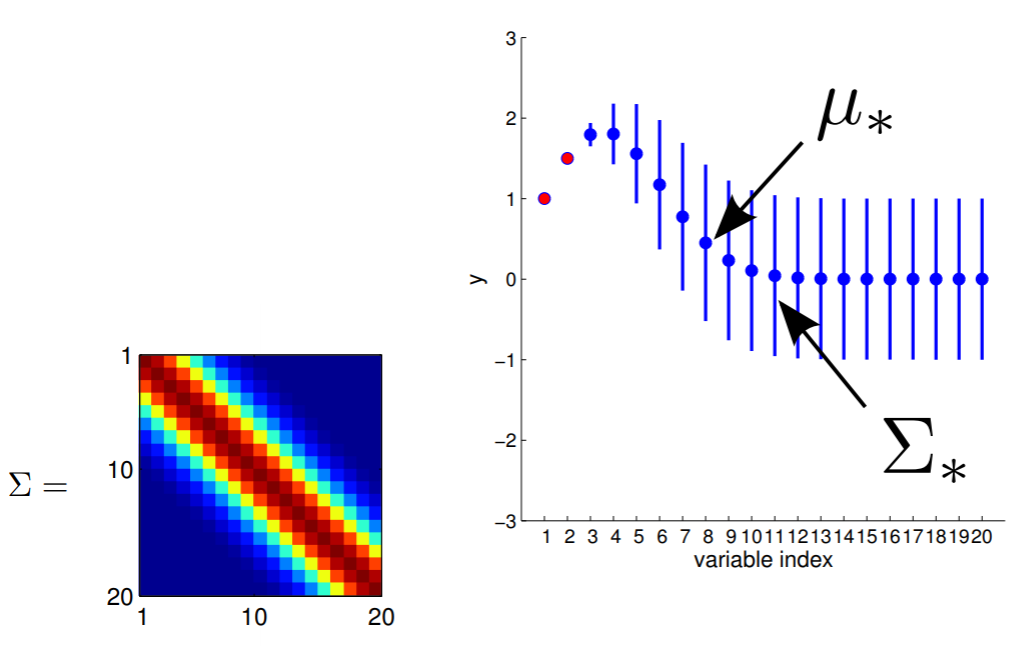
\includegraphics[width = .7\linewidth]{visualize2.png}
    \caption{Covariance matrix, calculated with the Radial Basis Function of equation \eqref{kernel} and the corresponding distribution of two sampled values with 18 values sampled from the normal distribution obtained using the covariance matrix.}
    \label{visual2}
\end{figure}

So in general for a Gaussian process we are only interested in two functions: a mean function $\mu(x)$ and a variance function $\sigma(x)$.
The mean function needs to pass from the points we sample at each iteration, the variance function tells us how uncertain we are about the value of the real function $f$ at given $x$. The example of what we want a Gaussian process to do is in Figure \ref{gp}. The points with a tick are the sampled values from the function. Clearly the mean passes through said points and the variance is almost zero nearby them whereas it becomes larger away from the sampled values because we are uncertain about the function at those test points. 

\begin{figure}
    \centering
    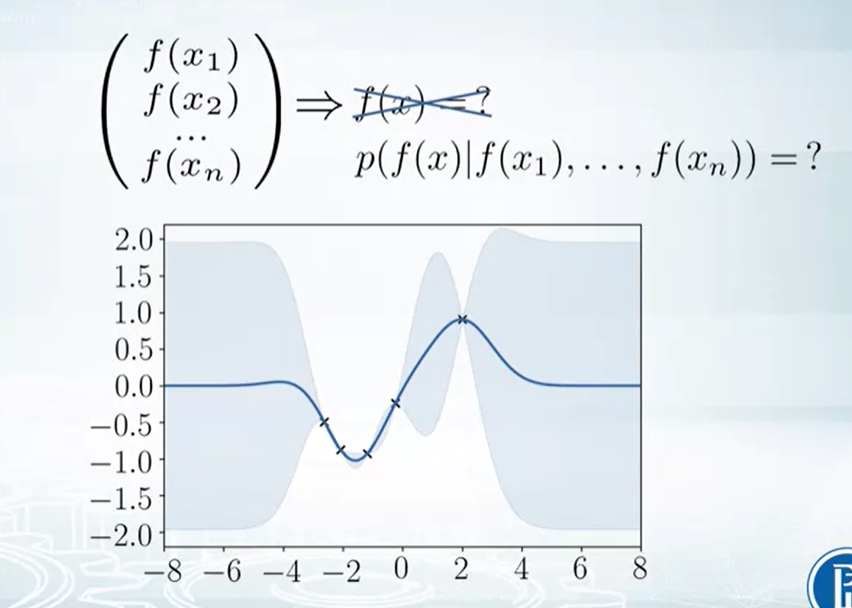
\includegraphics[width = .7\linewidth]{GPforML.png}
    \caption{Example of Gaussian Process}
    \label{gp}
\end{figure}

Finally it is important to choose the right kernel. The typical choice for the Kernel is the Radial Basis Function (RBF) which gives the gaussian weight to the distance of two points, aka:
\begin{equation}
    \label{kernel}
    \Tilde{\Sigma}(x_1 - x_2) = \sigma^2 \exp \big( - \frac{(x_1 - x_2)^2}{2l^2}\big)
\end{equation}
with $l$ the length scale of interaction and $\sigma$ the intensity. These are two hyperparameters that can be set with some optimization procedure that we do not care for right now. The meaning of this kernel is that we want variables with closer value of $x$ to be highly correlated. This makes the generated random gaussian functions very smooth. (being correlated for two variables $x_1$ and $x_2$ means that if $f(x_1) = 1.3$ then $f(x_2) \sim 1.3$ as well. While variables that are far apart can have very different variables. In this way we allow the sampled functions to be smooth and yet very wiggly (as wiggly as many variables we choose). 

\paragraph{Process}
Formally, we call a random process $f$ a Gaussian process if given any set of points $x_1, \dots, x_n \in R^d$ the joint distribution $f(x_1), \dots, f(x_n) \sim \mathcal{N}$ is a normal distribution. Any set of points means we can take $n \in \mathbb{N}$ and its the same for 1 or for a milion points. So we can use a limited number of sampling for our extimate. There are two functions of interest: The mean which is the expectation of the process $\mathbb{E}f(x) = m(x)$ and the covariance $Cov[f(x_1), f(x_2)] = \Sigma(x_1, x_2)$ which is obtained from a Kernel function.

So what we are doing is assuming that the variables for which we sample $f$ are not independent but are indeed correlated with each other and the correlation is given by the kernel function. So in general if we start with 10 different points we are assuming that those 10 points are 10 variables correlated to each other that generates functions gaussianly distributed. Meaning that I can assume mean 0 (or not if its different) I can use the kernel to calculate the correlation between these variables and from this I can sample as many functions as possible, only problem is that at first step they'll be very randomly distributed around the mean, as we already showed in the prior. 

Now we apply Bayesian learning. We have a training set $\mathcal{D} = \{(x_{TR}, f(x_{TR}))\}$ of $N$ tuples and our prior, our current belief on the unknown $f$, is that $f$ can be obtained by sampling a MVN that depends on our $N$ variables with mean 0 and variances given by the covariance matrix $\Sigma$ constructed with the kernel \eqref{kernel}:
\begin{equation}
    \begin{bmatrix}
    f(X_{TR}^{(1)}) \\
    f(X_{TR}^{(2)}) \\
    \vdots \\
    f(X_{TR}^{(N)})
    \end{bmatrix}
    \sim
    \mathcal{N}
    \begin{pmatrix}
    \begin{bmatrix}
    0 \\
    0 \\
    \vdots \\
    0
    \end{bmatrix}
    ,
    \begin{bmatrix}
    \Sigma_{11} & \Sigma_{12} & \dots & \Sigma_{1N} \\
    \Sigma_{21} & \Sigma_{22} & \dots  \\
    \vdots & \vdots{} & \ddots \\
    \Sigma_{N1} & \dots & \dots & \Sigma_{NN}
    \end{bmatrix}
    \end{pmatrix}
\end{equation}
Now we pick a value $x^\star$ (which is itself another nomally distributed variable with mean 0 and assumed variance 1) and if we want to know the value and confidence of the function $f^\star = f(x^\star)$ at that point we need to correlate $f^\star$ with $f(X_{TR})$, which we call $f$ for brevity, and this is done by creating a joint distribution like so:
\begin{align*}
    \begin{bmatrix}
    f \\
    f*
    \end{bmatrix}
    \sim
    \mathcal{N}
    \begin{pmatrix}
    \begin{bmatrix}
    0    \\    \vdots    \\    0
    \end{bmatrix}
    ,
    \begin{bmatrix}
    \begin{array}{c c c|c}
        \Sigma_{11} & \dots & \Sigma_{1N} & \Sigma_{1\star} \\
        \vdots &\ddots & \vdots & \vdots \\
        \Sigma_{N1} & \dots & \Sigma_{NN} & \Sigma_{N\star} \\
        \hline
        \Sigma_{\star 1} & \dots & \Sigma_{\star N} & \Sigma_{\star \star}
    \end{array}
    \end{bmatrix}
    \end{pmatrix}
    \sim
    \mathcal{N}
    \begin{pmatrix}
    \begin{bmatrix}
    0    \\    \vdots    \\    0
    \end{bmatrix}
    ,
    \begin{bmatrix}
    \begin{array}{c c c|c}
         &  & &  \\
         & \Sigma & & k_\star \\
         &  &  &  \\
        \hline
         & k^T_\star &  & \Sigma_{\star \star}
    \end{array}
    \end{bmatrix}
    \end{pmatrix}
\end{align*}
where we called $k_\star = (\Sigma_{1\star}, \dots, \Sigma_{N\star})$.
Using the MVN theorem we can calculate the mean and variance functions at the point $x_{\star}$:
\begin{align}
\label{GP}
    \mu(f^\star) &= \mu^\star = k_\star^T \Sigma^{-1} f \\
    \sigma(f^\star) &= \sigma^\star -k_\star^T \Sigma^{-1} k_\star + \Sigma_{\star \star}
\end{align}
which can be easily generalized to the case where $x_\star$ is a set of points by using the Cholesky decomposition to invert matrix $\Sigma$ for computational expense reasons. 

\subsection{Bayesian Optimization for function minimization}
Bayesian Optimization is a procedure used to learn a function or its extreme points by iteratively use the bayesian rule. It is used when the sampling of the function can be expensive in time or resources and thus we need to sample one (or only a few) point(s) at a time. So the assumption is to update the posterior as often as possible to gather information on where to sample next. 

The case we are interested in is the minimization (maximizing) of a function using a BO procedure and a Gaussian Process which is suited for the problem since it can be used to estimate the points where we are more unsure about the shape of the real function. We assume that at each iteration we have one (or a set of) new training points to add to the dataset $\mathcal{D} = (x_i, f(x_i))$. Then we use equations \eqref{GP} to gain a mean function and a variance function that gives our current knowledge of the real function to estimate, meaning that it is our posterior $p(f | \mathcal{D})$. The only thing to answer is what points to chose to sample the function $f$. 

\paragraph{Acquisition Function}
In general when looking for the next sampling point we need to balance two things:
\begin{enumerate}
    \item Exploration: this means look for sampling in areas where our current knowledge is scarse, \textit{i.e.} where the variance is low
    \item Exploitation: look for sampling in the area which currently has the lowest (largest) value.
\end{enumerate}
At every iteration we can find the current minimum/maximum value of the mean function, that is $\min \mu(x) = \mu^-$ for the minimum and $\max \mu(x) = \mu^+$ for the maximum, and then use an acquisition function that is large at the points where a new minima/maxima could be found. 

The most simple solution is called Probability of Improvement, PI, which is just a function that for every $x$ returns the probability that $f(x) \leq \mu^-$ or $f(x) \geq \mu^+$. For the maxima this is simply give by the cumulative distribution function (CDF) of the gaussian, $\phi$ at every point:
\begin{align}
    maxima: &PI(x) = P(f(x) > \mu^+) = \phi(\frac{\mu(x) - \mu^+}{\sigma(x)}) \\
    minima: &PI(x) = P(f(x) < \mu^-) = 1 - \phi(\frac{\mu(x) - \mu^+}{\sigma(x)})
\end{align}
The CDF $\phi$ is the right choice because it is close to zero for values that are much less than $\mu^+$ and 1 for values much larger. Clearly, for the minima, we do the opposite and thus we calculate 1 minus the CDF of the gaussian. 
The problem with the PI acquisition function is that it can be too greedy, it tends to search the new sample points around the current local minima/maxima, this is good for convex functions but it is not ideal for functions with complicated landscapes. 

Another very common option is called Expected Global Optimization or Expected Improvement (EI) and it is defined as the expectation value 
\begin{equation}
    \alpha(x) = \mathbb{E}[\max (0, f(x) - \mu^+ - \xi | \mathcal{D}]
\end{equation}
which is said to perform better than PI. It is implemented as:
\begin{equation}
    \alpha(x) = 
    \begin{cases}
        (\mu(x) - \mu^+) \phi \big( \frac{\mu(x) - \mu^+ - \xi}{\sigma(x)} \big) + \sigma(x) \mathcal{N}\big(\frac{\mu(x) - \mu^+ - \xi}{\sigma(x)}\big) & \text{for }\sigma(x) >0 \\    
        0 & \text{otherwise}   
    \end{cases}
\end{equation}

So putting altogether we have a valid algorithm to look for minima or maxima of a function, its flow is the following:
\begin{enumerate}
    \item Start with one, or a few, points $x_{TR}$. Sample the function at said points so that every point has label: $y_{TR} = f(x_{TR})$.
    \item Calculate $\Sigma$ using the training points $x_{TR}$.
    \item Calculate $ L = \sqrt{\Sigma}$ with Cholensky decomposition.
    \item Pick a set of test points $x_{TE}$, the more you pick the more precisely you can reconstruct the function. And then calculate:
    \begin{align}
        k_\star &= \Tilde{\Sigma}(x_{TR}, x_{TE}) \\
        \mathbf{y} &= L \backslash \mathbf{y}_{TR} \\
        \boldsymbol{\alpha} &= L^T \backslash \mathbf{y} \\
        \mathbf{v} &= L \backslash \mathbf{k}_\star
    \end{align}
    where $\mathbf{y}$ and $\mathbf{\alpha}$ is just a temp variable to calculate the inverse of $\Sigma$ through $L$ applied to $\mathbf{y}_{TR}$.
    \item Obtain the new mean and function at every test point with:
    \begin{align}
        \mu^\star &= \boldsymbol{k}_\star \cdot \boldsymbol{\alpha}\\
        \Sigma^\star &= \Tilde{\Sigma}(X_{TE}, X_{TE}) - \mathbf{v}^T \cdot \mathbf{v}
    \end{align}
    \item Evaluate the acquisition function at each test point
    \item Repeat process by sampling at the point with largest acquisition function value until convergence.
\end{enumerate}


\end{document}

